\section{Diverses}

\subsection{JSON-Tree}

\begin{lstlisting}[label=lst:JsonTree,caption=Json Struktur, language=JavaScript, style=htmlcssjs, mathescape]
{
  "product": "api.wetter-arbon.ch",
  "version": "1.1.1",
	{
    "v1": {
        "misc": {
            "west": {
                "description": "Warnlevel west",
                "warnlevel": 40,
                "onset": "2018-07-17 13:05:00",
                "expires": null,
                "timestamp": "2018-07-17 13:24:00",
                "interval": 60,
                "intervalUnit": "seconds"
            },
            "middle": {
                "description": "Warnlevel middle",
                "warnlevel": 40,
                "onset": "2018-07-17 13:06:00",
                "expires": null,
                "timestamp": "2018-07-17 13:24:00",
                "interval": 60,
                "intervalUnit": "seconds"
            },
            "east": {
                "description": "Warnlevel east",
                "warnlevel": 0,
                "onset": null,
                "expires": null,
                "timestamp": "2018-07-17 13:24:00",
                "interval": 60,
                "intervalUnit": "seconds"
            }
        },
        "webcam": {
            "name": "Webcam Wetter Arbon",
            "title": "webcam",
            "url": "https://webcam.wetter-arbon.ch/mjpg/video.mjpg"
        },
        "data": {
            "temperature": {
                "description": "Lufttemperatur",
                "unit": "${^\circ}$C",
                "value": 22.6,
                "dailymax": 22.6,
                "dailymin": 17,
                "timestamp": "2018-07-17 13:24:31",
                "interval": 60,
                "intervalUnit": "seconds"
            },
            "windchill": {
                "description": "Windchill",
                "unit": "${^\circ}$C",
                "value": 22.6,
                "dailymax": 22.6,
                "dailymin": 17,
                "timestamp": "2018-07-17 13:24:31",
                "interval": 60,
                "intervalUnit": "seconds"
            },
            "humidity": {
                "description": "Relative Luftfeuchtigkeit",
                "unit": "%",
                "value": 60,
                "timestamp": "2018-07-17 13:24:31",
                "interval": 60,
                "intervalUnit": "seconds"
            },
            "winddirection": {
                "description": "Windrichtung",
                "unit": "${^\circ}$",
                "value": 75,
                "timestamp": "2018-07-17 13:24:31",
                "interval": 60,
                "intervalUnit": "seconds"
            },
            "windspeed": {
                "knoten": {
                    "value": 7.6,
                    "dailymax": 7.9,
                    "unit": "kn"
                },
                "kmph": {
                    "value": 14.08,
                    "dailymax": 14.63,
                    "unit": "km/h"
                },
                "beaufort": {
                    "value": 3,
                    "dailymax": 3,
                    "unit": "Bft"
                },
                "description": "Windgeschwindigkeit",
                "timestamp": "2018-07-17 13:24:31",
                "interval": 60,
                "intervalUnit": "seconds"
            },
            "gust": {
                "knoten": {
                    "value": 8,
                    "dailymax": 8.2,
                    "unit": "kn"
                },
                "kmph": {
                    "value": 14.82,
                    "dailymax": 15.19,
                    "unit": "km/h"
                },
                "beaufort": {
                    "value": 3,
                    "dailymax": 3,
                    "unit": "Bft"
                },
                "description": "Böen",
                "unit": "kn",
                "timestamp": "2018-07-17 13:24:31",
                "interval": 60,
                "intervalUnit": "seconds"
            },
            "precipitation": {
                "description": "Niederschlagsmenge seit Mitternacht",
                "unit": "mm",
                "value": 0,
                "timestamp": "2018-07-17 13:24:31",
                "interval": 60,
                "intervalUnit": "seconds"
            },
            "pressure": {
                "description": "Luftdruck",
                "unit": "hPa",
                "value": 1017.1,
                "timestamp": "2018-07-17 13:24:31",
                "interval": 60,
                "intervalUnit": "seconds"
            },
            "weathericon": {
                "description": "Icon type current weather",
                "value": 5,
                "timestamp": "2018-07-17 13:24:31",
                "interval": 60,
                "intervalUnit": "seconds"
            },
            "forecasticon": {
                "description": "Forecast icon",
                "value": 5,
                "timestamp": "2018-07-17 13:24:31",
                "interval": 60,
                "intervalUnit": "seconds"
            },
            "watertemperature1m": {
                "description": "Wassertemperatur 1m unter der Wasseroberfläche",
                "unit": "${^\circ}$C",
                "value": 24.2,
                "timestamp": "2018-07-17 13:24:00",
                "interval": 60,
                "intervalUnit": "seconds"
            },
            "watertemperature0m5": {
                "description": "Wassertemperatur 0.5m unter der Wasseroberfläche",
                "unit": "${^\circ}$C",
                "value": 23.9,
                "timestamp": "2018-07-17 13:24:00",
                "interval": 60,
                "intervalUnit": "seconds"
            },
            "waterlevel": {
                "description": "Bodenseepegel",
                "unit": "m",
                "value": 3.54,
                "timestamp": "2018-07-17 13:24:00",
                "interval": 60,
                "intervalUnit": "seconds"
            },
            "radiation": {
                "description": "Globalstrahlung",
                "unit": "W/m2",
                "value": 868,
                "timestamp": "2018-07-17 13:24:00",
                "interval": 60,
                "intervalUnit": "seconds"
            },
            "sunduration": {
                "description": "Sonnenstunden",
                "unit": "h/d",
                "value": 5,
                "timestamp": "2018-07-17 13:24:00",
                "interval": 60,
                "intervalUnit": "seconds"
            }
        }
    }
}
}
\end{lstlisting}

\subsection{Datenbankcode}\label{anhang:Datenbankcode}
\begin{itemize}
	\item API
	\item Links? (URL, Git, GitPages, usw.)
\end{itemize}


% Subscection
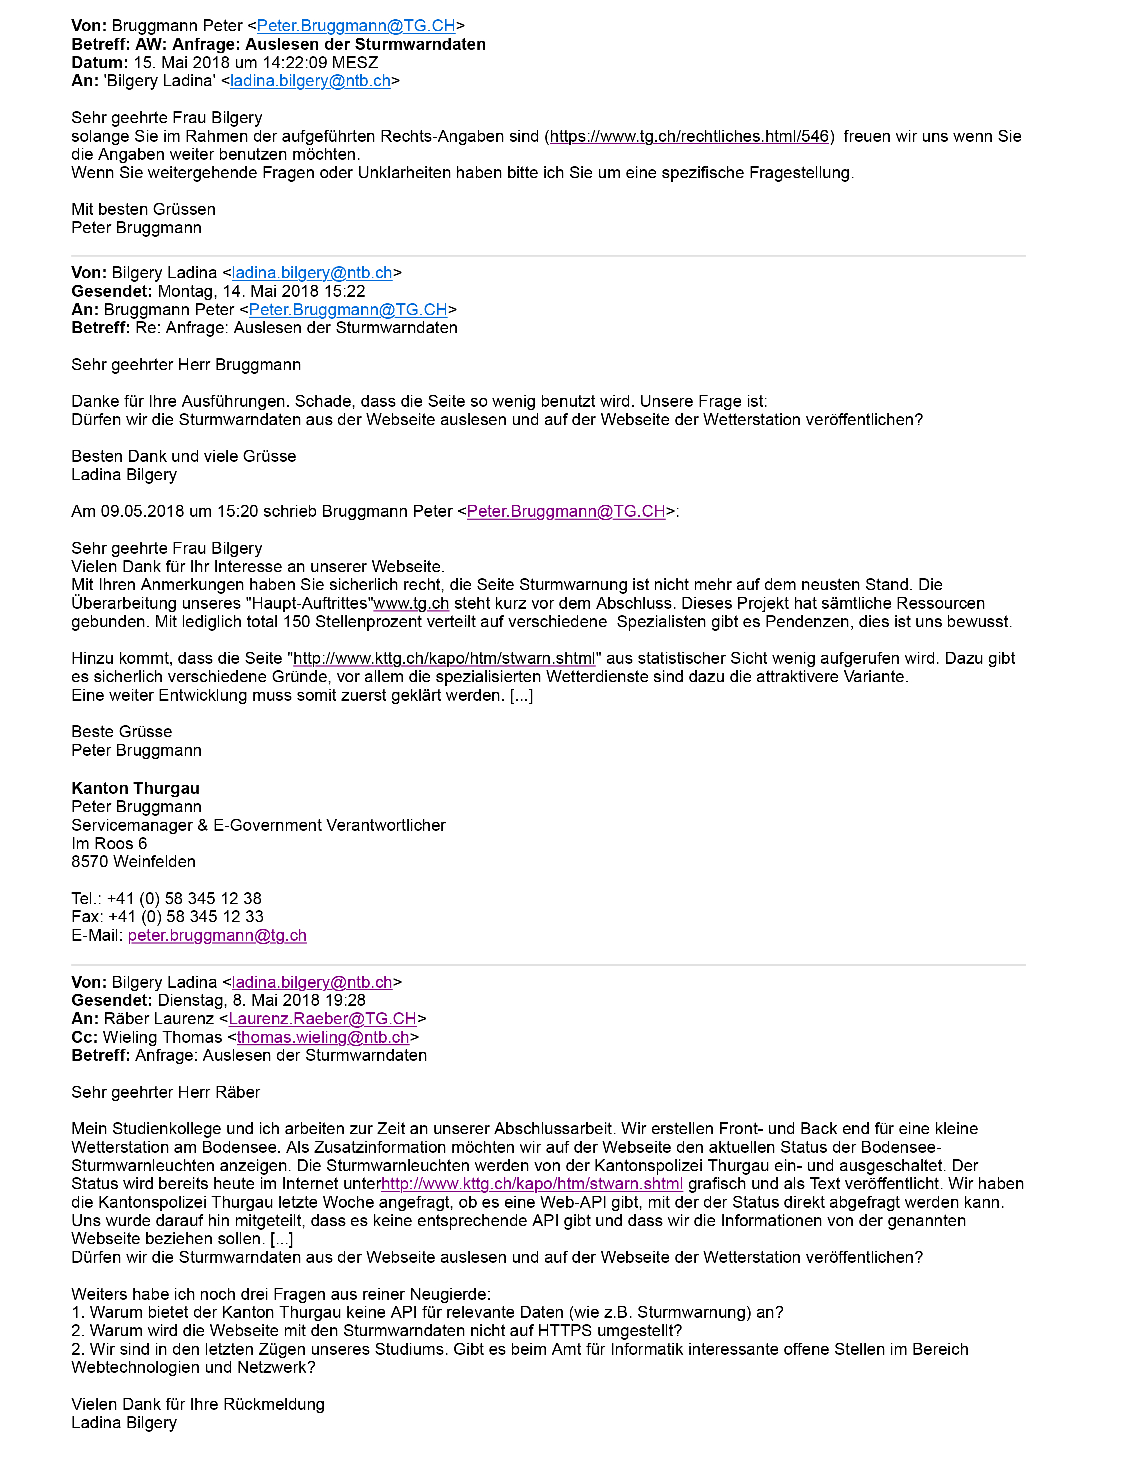
\includepdf[pages=-,frame,scale=0.7,pagecommand={\pagestyle{plain}\subsection{Bestätigungs-E-Mail des Amts für Informatik Thurgau}\label{anhang:email}}]{appendix/email.pdf}
